\documentclass[12pt]{article}

\usepackage[utf8]{inputenc}
\usepackage[portuguese]{babel}
\usepackage{float}
\usepackage{graphicx}
\usepackage{amssymb}

\title{MAC0444 - Sistemas Baseados em Conhecimento \\
Lista de Exercícios No. 2
}
\author{Mateus Agostinho dos Anjos\\NUSP 9298191}
\date{\today}

\begin{document}
	\maketitle
	\begin{itemize}
		\item[\textbf{1 -}]
			\hfill\newline
			Predicados:\\
			$fezEx(x)$ = x fez os exercícios\\
			$vaiBem(x)$ = x vai bem na prova\\
			$mediaAlta(x)$ = x fica com media alta\\
			$aprovado(x, y)$ = x é aprovado em y \\
			\newline
			Formalizando as sentenças do enunciado chegamos em:\\
			$$\forall x \ (fezEx(x) \rightarrow vaiBem(x))$$
			$$\forall y \ (vaiBem(y) \rightarrow mediaAlta(y))$$
			$$\forall z \ (mediaAlta(z) \rightarrow aprovado(z, mac444))$$
			$$fezEx(\textnormal{João})$$
			$$vaiBem(\textnormal{Maria})$$
			Base de conhecimento (KB):\\
			\begin{center}
				\begin{tabular}{c l}
				1. & $[\neg fezEx(x), \ vaiBem(x)]$\\
				2. & $[\neg vaiBem(y), \ mediaAlta(y)]$\\
				3. & $[\neg mediaAlta(z), \ aprovado(z, mac444)] $\\
				4. & $[fezEx(\textnormal{João})]$\\
				5. & $[vaiBem(\textnormal{Maria})]$\\
				6. & $[\neg aprovado(\textnormal{João}, mac444)]$\\
				\end{tabular}
			\end{center}
			Veja que inserimos $[\neg aprovado(\textnormal{João}, mac444)]$ na base de 
			conhecimento, pois	é a negação do nosso objetivo. Sendo assim, se chegarmos na 
			cláusula vazia a partir desta base de conhecimento estará provado que 
			$aprovado(\textnormal{João}, mac444)$ é consequência lógica das sentenças do
			 enunciado.\\
			\newline
			Utilizando a \textbf{resolução SLD} temos:\\
			\begin{center}
				\begin{tabular}{c c}
					$\neg aprovado(\textnormal{João}, mac444)$ & (resolve com 3. e z/João)\\
					$\downarrow$ & \\
					$\neg mediaAlta(\textnormal{João})$ & (resolve com 2. e y/João)\\
					$\downarrow$ & \\
					$\neg vaiBem(\textnormal{João})$ & (resolve com 1. e x/João)\\
					$\downarrow$ & \\
					$\neg fezEx(\textnormal{João})$ & (resolve com 4.)\\
					$\downarrow$ & \\
					$[ \ ]$ & \\
				\end{tabular}
			\end{center}
			Sendo assim provamos que: $KB \ \cup \  \{ \neg aprovado(\textnormal{João}, 
			mac444) \}$ é insatisfazível, portanto $aprovado(\textnormal{João}, mac444)$  
			é consequência lógica de nossa base de conhecimento.\\ \\
			A \textbf{resolução SLD} será semelhante para Maria, portanto temos:\\
			Base de conhecimento (KB):\\
			\begin{center}
				\begin{tabular}{c l}
				1. & $[\neg fezEx(x), \ vaiBem(x)]$\\
				2. & $[\neg vaiBem(y), \ mediaAlta(y)]$\\
				3. & $[\neg mediaAlta(z), \ aprovado(z, mac444)] $\\
				4. & $[fezEx(\textnormal{João})]$\\
				5. & $[vaiBem(\textnormal{Maria})]$\\
				6. & $[\neg aprovado(\textnormal{Maria}, mac444)]$\\
				\end{tabular}
			\end{center}
			Utilizando a \textbf{resolução SLD} temos:\\
			\begin{center}
				\begin{tabular}{c c}
					$\neg aprovado(\textnormal{Maria}, mac444)$ & (resolve com 3. e z/Maria)\\
					$\downarrow$ & \\
					$\neg mediaAlta(\textnormal{Maria})$ & (resolve com 2. e y/Maria)\\
					$\downarrow$ & \\
					$\neg vaiBem(\textnormal{Maria})$ & (resolve com 5.)\\
					$\downarrow$ & \\
					$[ \ ]$ & \\
				\end{tabular}
			\end{center}
		\item[\textbf{2 -}]
			\hfill\newline
			Temos a Base de Conhecimento (KB) reescrita com variáveis renomeadas para evitar 
			confusões	na resolução do exercício:
			\begin{center}
				\begin{tabular}{c l}
				1. & $[\neg A_1(x), \neg A_2(x), P(x)]$\\
				2. & $[\neg B_1(y), \neg B_2(y), A_1(y)]$\\
				3. & $[\neg B_3(z), \neg B_4(z), A_2(z)]$\\
				4. & $[B_1(a)]$\\
				5. & $[B_2(a)]$\\
				6. & $[B_3(a)]$\\
				7. & $[B_4(a)]$\\
				\end{tabular}
			\end{center}
			\begin{itemize}	
				\item[\textbf{a) }]					
					\hfill\newline
					Para mostrar o passo a passo do procedimento de encadeamento para
					trás (backward chaining) devemos começar identificando as implicações
					da Base de Conhecimento.\\
					Seguindo a ordem acima temos:\\ 
					(note que utilizamos $\leftarrow$ nas implicações)\\
					\begin{center}
						\begin{tabular}{c l}
							1. & $\forall x (P(x) \leftarrow A_1(x) \land A_2(x))$\\
							2. & $\forall y (A_1(y) \leftarrow B_1(y) \land B_2(y))$\\
							3. & $\forall z (A_2(z) \leftarrow B_3(z) \land B_4(z))$\\
							4. & $B_1(a)$\\
							5. & $B_2(a)$\\
							6. & $B_3(a)$\\
							7. & $B_4(a)$\\
						\end{tabular}
					\end{center}
					A partir destas implicações o passo a passo pode ser mostrado a partir da figura
					abaixo, sendo que cada passo gera pelo menos uma sub-árvore.\\
					\begin{figure}[H]
						 	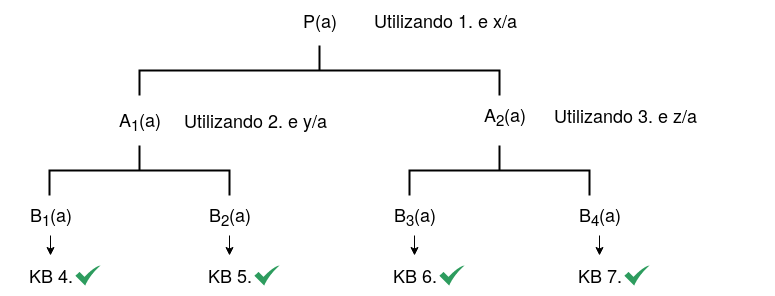
\includegraphics[scale=0.64]{backward_2a.png}
					\end{figure}
					\hfill\newline
					Todas as folhas da árvore estão na base de conhecimento em uma cláusula 
					unitária, portanto são verdadeiras. Sendo assim podemos marcá-las com um 
					\checkmark.\\
					A partir disso podemos concluir que $A_1(a)$ e $A_2(a)$ estão
					provados e depois que $P(a)$ está provado, portanto mostramos que o
					encadeamento para trás (backward chaining) produz resposta SIM com 
					objetivo P(a).
				\item[\textbf{b) }]
					\hfill\newline
					Utilizando a \textbf{resolução SLD} com a base de conhecimento definida
					no início da questão, iniciamos com $\neg P(a)$, que é a negação do nosso
					objetivo, e buscaremos a cláusula vazia.\\
					Obtemos o seguinte:\\
					\begin{center}
						\begin{tabular}{c c}
							$[\neg P(a)]$ & (resolve com 1. e x/a)\\
							$\downarrow$ & \\
							$[\neg A_1(a), \neg A_2(a)]$ & (resolve com 2. e y/a)\\
							$\downarrow$ & \\
							$[\neg B_1(y), \neg B_2(y), \neg A_2(a)]$ & (resolve com 3. e z/a)\\
							$\downarrow$ & \\
							$[\neg B_1(a), \neg B_2(a), \neg B_3(a), \neg B_4(a)]$ & (resolve com 4.)\\
							$\downarrow$ & \\
							$[\neg B_2(a), \neg B_3(a), \neg B_4(a)]$ & (resolve com 5.)\\
							$\downarrow$ & \\
							$[\neg B_3(a), \neg B_4(a)]$ & (resolve com 6.)\\
							$\downarrow$ & \\
							$[\neg B_4(a)]$ & (resolve com 7.)\\
							$\downarrow$ & \\
							$[ \ ]$ & \\
						\end{tabular}
					\end{center}
					\hfill\newline
					Como chegamos na cláusula vazia a partir de $\neg P(a)$, então está provado 
					que $P(a)$ é consequência desta base de conhecimento.
			\end{itemize}
		\item[\textbf{3 -}]
			\hfill\newline
			\begin{itemize}
				\item[\textbf{a) }]
					\hfill\newline
					Após ter carregado o programa a resposta do Prolog para a consulta:\\
					$?- result([a , b , c , d , e , f , g], X ).$\\
					será:\\
					$X = [b, d, f]$
				\item[\textbf{b) }]
					\hfill\newline
					Considerando que a lista é enumerada a partir da posição 1, o programa recebe
					uma lista e elimina os elementos das posições ímpares, devolvendo apenas
					os elementos das posições pares.\\
					Veja o exemplo de consulta que os elementos da lista coincidem com o número 
					de sua posição:\\
					$?- result([1, 2, 3, 4, 5, 6], X ).$\\
					$X = [2, 4, 6]$\\
					Para fazer isso o programa possui um fato, $result(\_, [ \ ])$, que cobre os
					casos em que o primeiro argumento é uma lista vazia ou uma lista com apenas
					1 elemento, pois nestes casos não é possível extrair 2 elementos da lista
					como a primeira regra exige (o corte impede a utilização do fato quando
					a lista tem 2 ou mais elementos).\\
					Definida a base do programa a partir deste fato, chamadas recursivas serão
					feitas tentando equiparar, inicialmente, a lista passada como argumento e a 
					primeira regra, veja a execução do exemplo:\\ \\
					\begin{tabular}{ll}
						Chamada inicial & $result([1, 2, 3, 4, 5, 6], X)$\\
						Casa com & $result([\_, E | L], [E | M])$\\
						Com valoração & $\_ = 1$, $E = 2$, $L = [3, 4, 5, 6]$, $X = [2|M_1]$\\
						Faz chamada recursiva & $result(L, M_1)$\\ \\
						
						Chamada & $result([3, 4, 5, 6], M_1)$\\
						Casa com & $result([\_, E | L], [E | M])$\\
						Com valoração & $\_ = 3$, $E = 4$, $L = [5, 6]$, $M_1 = [4|M_2]$\\
						Faz chamada recursiva & $result(L, M_2)$\\ \\
						
						Chamada & $result([5, 6], M_2)$\\
						Casa com & $result([\_, E | L], [E | M])$\\
						Com valoração & $\_ = 5$, $E = 6$, $L = [ \ ]$, $M_2 = [6|M_3]$\\
						Faz chamada recursiva & $result(L, M_3)$\\ \\
						
						Chamada & $result([ \ ], M_3)$\\
						Casa com o fato & $result(\_, [ \ ])$\\
						Com valoração & $\_ = [ \ ]$, $M_3 = [ \ ]$\\
					\end{tabular}
					\hfill\newline
					Após essa execução devemos obter o valor de $X$, para isso
					temos que reconstruí-lo a partir de $M_3$, $M_2$ e $M_1$, veja:\\
					\begin{tabular}{lll}
						$M_3$ = & $[ \ ]      $ & = [ \ ]\\
						$M_2$ = & $[6|M_3]$ & = [6]\\
						$M_1$ = & $[4|M_2]$ & = [4, 6]\\
						$X$     = & $[2|M_1]$ & = [2, 4, 6]\\
					\end{tabular}
					\hfill\newline\newline
					Esta execução única só é possível, pois o corte (!) na primeira linha do
					programa faz com que não seja possível criar ramificações para obter
					diferentes respostas casando as chamadas recursivas intermediárias 
					com o fato, uma vez que já foi utilizado a primeira regra de casamento 
					(que possui a instrução de corte).\\
					Sendo assim, o corte impede a alternativa de resposta em que o programa 
					casa 	a chamada $result([3, 4, 5, 6], M_1)$ com o fato $result(\_, [ \ ])$ 
					($\_ = [3, 4, 5, 6]$ e $M_1 = [ \ ]$) e obtém a resposta $X = [2]$, por 
					exemplo.\\
					Note que foi utilizado a variável anônima ($ \_$), pois não queremos
					saber qual o valor do elemento que foi atribuído a ela durante o
					processo de obtenção do valor de $X$, queremos somente que exista
					um valor possível a ser atribuído.
			\end{itemize}
		\item[\textbf{4 -}]
			\hfill\newline
			\begin{itemize}
				\item[\textbf{a) }]
				\item[\textbf{b) }]
				\item[\textbf{c) }]
				\item[\textbf{d) }]
				\item[\textbf{e) }]
				\item[\textbf{f) }]
				\item[\textbf{g) }]
				\item[\textbf{h) }]
				\item[\textbf{i) }]
				\item[\textbf{j) }]
			\end{itemize}
	\end{itemize}
\end{document}